
\section{Introduction}
The trading of stock shares can be triggered by high complex event patterns that are specified
based on patterns in the event stream of the stock market. Complex patterns are are specified based on the history of 
the event stream, for example, by utilizing moving averages of stock prices and the trading volumes.
The real-time extraction of such complex patterns to trigger buy or sell trading actions is the task
of high-performance event stream processing systems.

% Describe briefly what the challenge is
The 2022 DEBS Grand Challenge \cite{debs2022challenge} describes a system implementation based on two specific queries on the
stock market event streams. The first query is defined to compute the Exponential Moving Average (EMA) with two different smoothing factors of 38 and 100.
An exponential Moving Average is one of the moving averages and is defined as follows:

\begin{align*}
    EMA_t = \begin{cases}
        Y_0 &  t = 0 \\
        \alpha Y_t + (1-\alpha) EMA_{t-1}& t>0 \\
        \end{cases}
\end{align*}

The coefficient $\alpha$ represents the degree of weighting decrease, a constant smoothing factor between 0 and 1.
For this challenge $\alpha = \frac{2}{1+j}$ where $j$ is a smoothing factor with $j \in \{38, 100 \}$.
We use $EMA_{38}$ to refer to the exponential moving average with a smoothing factor of 38 and $EMA_{100}$ for a smoothing factor of 100.


\begin{figure}[!ht]
    \begin{center}
        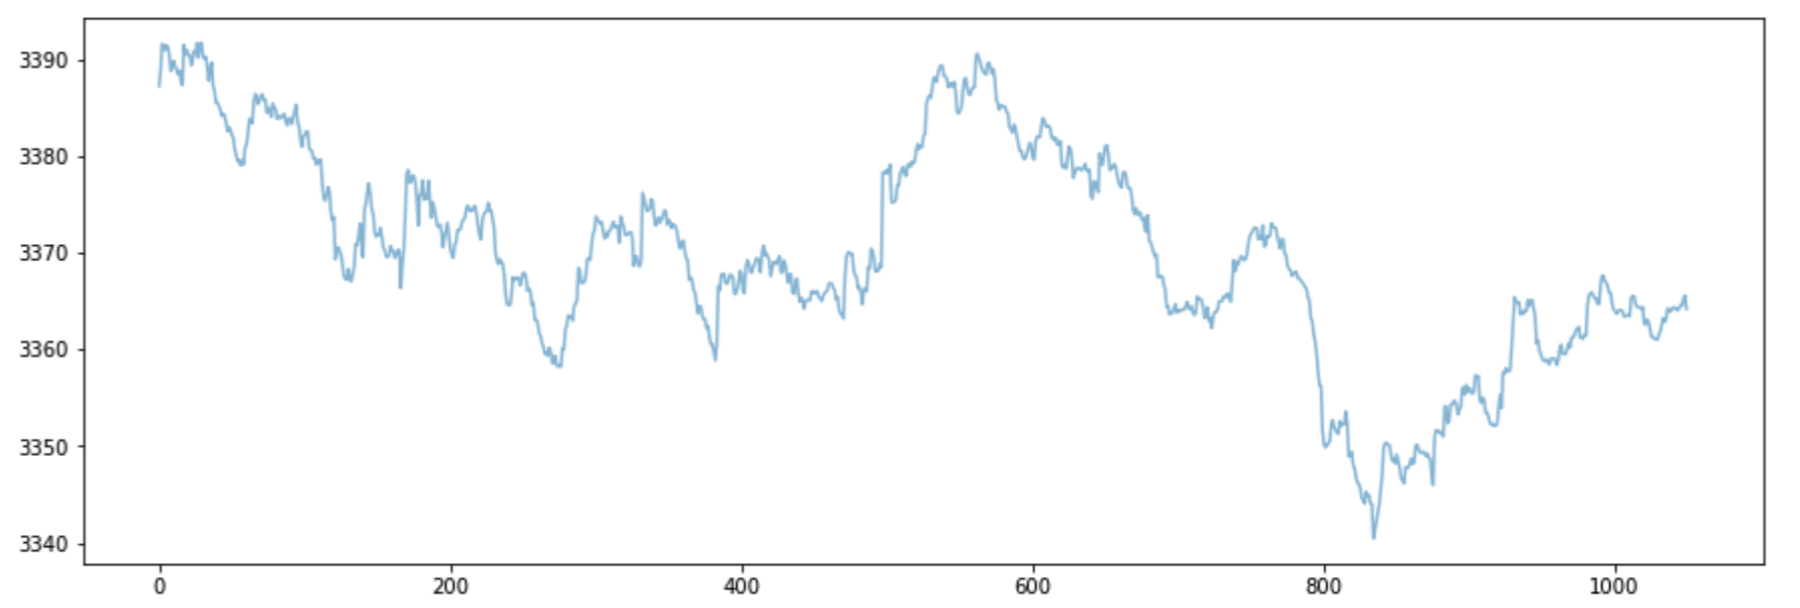
\includegraphics[width=0.42\textwidth]{./images/stock_example.png}
        \caption{An Example of Stock Price Fluctuations Over Time}
        \label{fig:stock}
    \end{center}
\end{figure}



\begin{figure*}[!ht]
    \begin{center}
        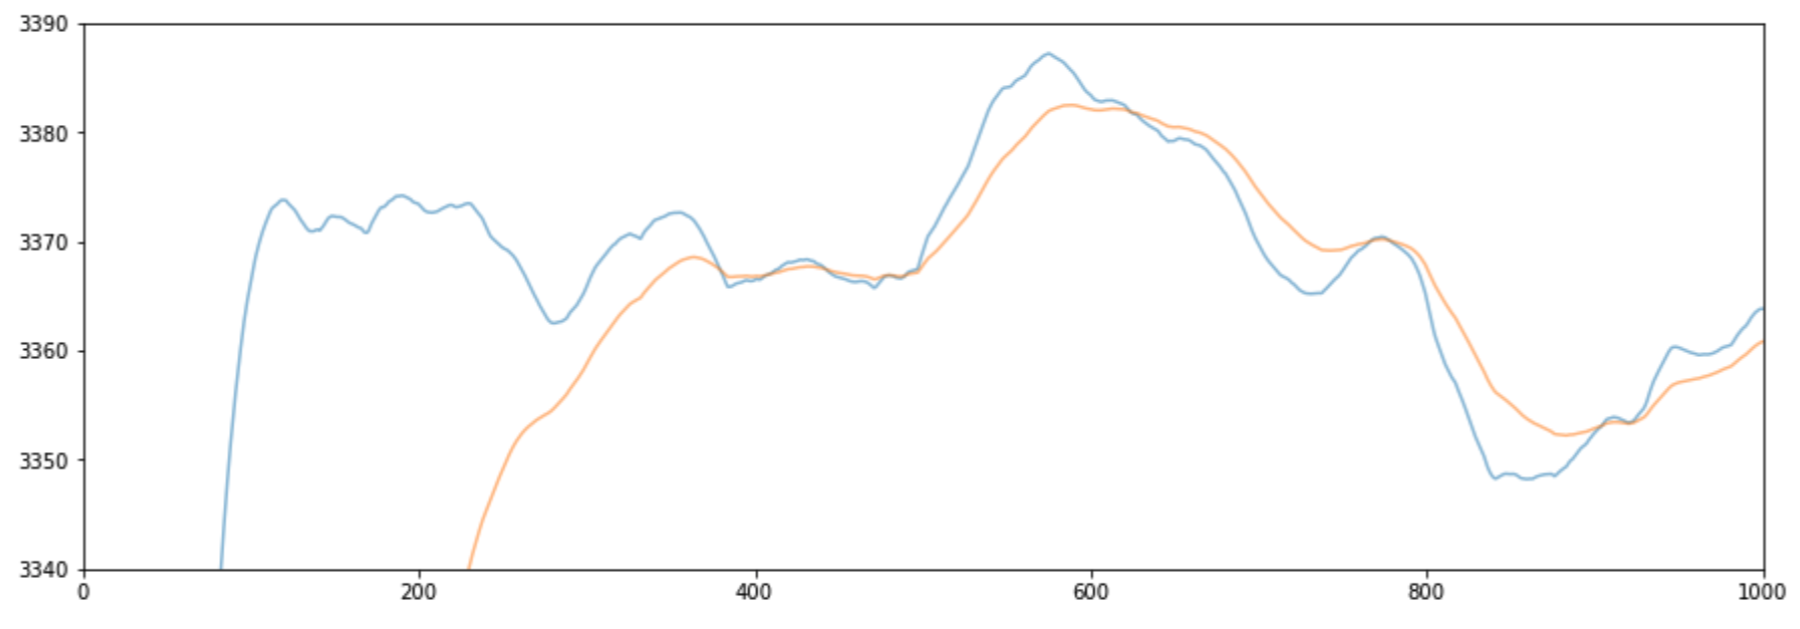
\includegraphics[width=0.70\textwidth]{./images/query2_example.png}
        \caption{Example of Query 2 - Buy and Sell advice based on Breakout Patterns of EMA 38 and 100 }
        \label{fig:EMAs}
    \end{center}
\end{figure*}


% Describe the query 1 and 2
Figure \ref{fig:stock} illustrates an example of stock market price changes over time. The graph shows 1000 events with
different prices. Figure \ref{fig:EMAs} depicts the values of the exponential moving average with
smoothing factors of 38 and 100. We can observe in Figure \ref{fig:EMAs} how the value grows exponentially
and how the two $EMA_{38}$ and $EMA_{100}$ are different from each other.

Query 2 of the DEBS 2022 challenge \cite{debs2022challenge} is specified based on the results of Query 1. Each time
that $EMA_{38}$ breaks out of the value of $EMA_{100}$ a stock buy advice notification should be generated and if
$EMA_{100}$ goes under the $EMA_{38}$ a stock sell advice. For a further detailed description of the DEBS 2022
Grand Challenge, we would refer the readers to \cite{debs2022challenge}.

Figure \ref{fig:EMA200} visualizes the same graph as we have in Figure \ref{fig:EMAs} by
zooming into the graph (range 0 to 400 events on x-axis) to see the values and their differentiations. One important observation in
Figures \ref{fig:EMA200} and \ref{fig:EMAs} is that $EMA_{38}$ and $EMA_{100}$ have a large difference in the first
200 events.  The reason for this difference is that the exponential moving average is specified based
on the history of events to increase the value exponentially and requires a warm-up phase. Based on this observation,
one can improve the performance of the Query 2 by skipping the first 200 events because
$EMA_{38}$ and $EMA_{100}$ still have a large difference.

The main system development challenge task is to design a system that can process the stream of events with high throughput and low latency.
Many open source and commercial stream processing systems are developed that one can use to develop this challenge.
Esper event stream processing system \cite{Bernhardt2007} is a system that can detect complex events based on pre-defined temporal logic patterns.
In this task we do not have a complex pattern to extract and computations are basic computations of EMA 38 and 100, following with a check of the values for
Query 2 to submit a sell or buy advice. Other systems like Apache Storm \cite{8288619}, Apache Spark Streaming \cite{zaharia2010spark} or
Apache Flink streaming \cite{alexandrov2014stratosphere} have been developed to achieve high-scalability in data stream processing.
Also, different benchmarks are developed \cite{8701904} which compare these systems with each other regarding specific data
stream processing tasks.

After considering all of the existing systems and their overhead trade-offs, we decided to implement the DEBS Grand Challenge from scratch,
without using any of the existing systems like Apache Spark or Flink. Most of these systems have a different target like higher scalability than higher performance, so that 
they have a large start-up delay and additional cluster management costs. 

% https://asterios.katsifodimos.com/assets/publications/flink-deb.pdf

Some examples of the performance overheads that systems like Apache Spark and Flink have are:

\begin{itemize}
    \item Most of the systems are designed in a distributed cluster computing setting which include cluster managements like communications between the master process/es and worker processes.
    Separate processes are started as JobManager and TaskManager to coordinate different task executions. 

    \item These systems are designed for the trade-off between higher scalability and higher stream throughput/latency performance. 
    The described DEBS 2022 challenge does not include a very large  data stream that we would need to design a high-scalable data stream processing system. But our main system design goal is to achieve 
    high-throughput and low-latency. Systems like Spark or Flink include internal data processing pipelines including batch processing and blocking data exchanges. 
    
    \item Such systems use special types of control events, like  checkpoint barriers, watermarks signaling or iteration barriers to be able to generate snapshots of 
    the data stream for example to provide guarantee a FIFO order of events and be able to do stream recovery \cite{df177547a4364bb0a7e2470b83025bb0}. 
    In our from scratch implementation, we can make sure that our stream processing is stateful and windows are correctly generated from the stream batches.

    \item The cluster stream processing systems have a lots of configuration parameters to modify the cluster settings. 
    For example these configurations control number of cluster executor processes and threads. To achieve highest performance, we would need 
    to experiment a lot to set the system to highest throughput and latency performance. 
    With our from scratch implementation, we can better control the system parameters like number of processes or threads. 

    \item The DEBS Challenge queries are very simple patterns that we can implement in a programming language, and there is no need to have a complex query processing and query optimization system. 

\end{itemize}


First, we implemented the two data stream queries as a prototype system in python and run tests to check if the data streams are processed correctly, and the correct
results are submitted to the DEBS 2022 evaluation system. In the second project phase we implemented the same system in Java to achieve better processing 
performance (a better performance can be achieved by using a system language like C++ or Rust).  
Our implementation in Python and Java are available on Github\footnote{\url{https://github.com/kiat/debs2022} last update June, 2022}


% High-Performance computing problems
% Scalability issues

\begin{figure}[!ht]
    \begin{center}
        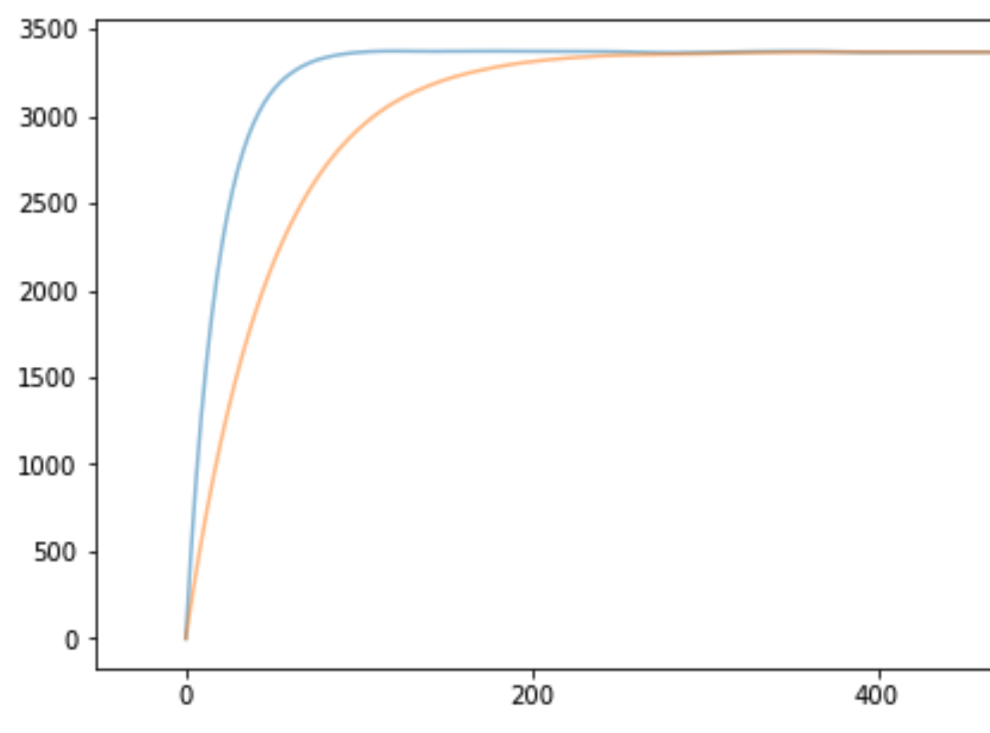
\includegraphics[width=0.4\textwidth]{./images/query2_example_200.png}
        \caption{Exponential Moving Average of 38 and 100 for the first 400 events.}
        \label{fig:EMA200}
    \end{center}
\end{figure}


The next subsequent sections describe details of our implementation. Section \ref{sec:concepts} describes our conceptual design for
a stream processing system using multiple processing threads on a single machine with multiple CPU cores. Further we describe how the same
architecture can be extended to process the data stream on a cluster of machines (multi-processing).  Section \ref{sec:implementation} provides
a brief description of important implementation details and Section \ref{sec:experiments} provides a brief overview of example
experiment results.
